\section{Results and Discussion}
\label{sec:results}
In this section we presented the findings derived from applying MTGNN, and other baseline forecasting methods. Before starting analyses, all historical data values were transformed to natural logarithm. The initial $60\%$ of 
the dataset used for training the models, the subsequent $20\%$ of the data was used for validation and the last $20\%$ of the data, starting from January 2022 and ending on August 14, 2024 were used for testing purposes.

All the hyperparameters of the MTGNN used to obtain the results are summarized in Table~\ref{tab:hyperparams}. 

\begin{table}[bt]
    \caption{The hyperparameters of the MTGNN used to train and infer the forecasts.}
    \label{tab:hyperparams}
    \centering
    \begin{tabular}{ *3l }           \toprule
    \emph{Hyperparameter}  & \emph{Value} \\ \cmidrule(lr){1-2}
    Convolution depth & $2$ \\
    Loss & $\ell_1$ \\
    Dropout & $0.3$ \\
    Convolutional channels & $16$ \\
    Residual channels & $16$ \\
    Skip channels & $32$ \\
    Batch size & $8$ \\ 
    Epochs & $30$ \\
    \bottomrule
    \hline
    \end{tabular}
\end{table}
%

Once the MTGNN training phase was performed, the constructed graph was shown in Figure~\ref{fig:graph}. In the graph, each node represents the countries' stock indices, and each edge represents the link between them.
In this study, we used a convolutional graph network with depth $2$. This means that each node had their feature vector updated by considering the current information 
residing in its $2$-hop neighborhood \textit{(i.e., its neighbors and the neighbors of its neighbors)}.
The constructed graph should be understood in the sense that 2-hop neighbors have a direct effect 
on the outcome of each node, and others may only have an indirect effect in predicting the future 
values of a particular node. Notice that this graph is constructed by performing and end-to-end 
stochastic gradient descent (more precisely, the Adam optimizer), on the losses accrued between 
the predicted and the actual values. This means that by no means do we claim that the constructed 
graph in Figure~\ref{fig:graph}, is a causal one. It is the graph that the optimization has 
constructed such that the resulting loss is minimized. 

The adjacency matrix, corresponding to 
the graph in Figure~\ref{fig:graph} is given by \textbf{A}. The matrix provides a visual representation of the connections and their strengths between the countries' stock indices. Zeros in the matrix demonstrate no connection between them. According to the adjacency matrix and Figure~\ref{fig:graph}, when we only consider 1-hop neighborhoods, among G7 countries, the US's \textit{(with 7 out-degree connections)}, Germany's and Canada's \textit{(with 5 out-degree connections)} stock indices and among MINT countries, Indonesia's \textit{(with 7 out-degree connections)} and T\"{u}rkiye's \textit{(with 6 out-degree connections)} stock indices are the most influential ones in the forecasting process. If we consider 2-hop neighborhoods as determined, according to the $\bm{A}^2$ matrix, among G7 countries, the US's \textit{(with 39 out-degree connections)} and Canada's \textit{(with 34 out-degree connections)} stock indices, and among MINT countries, Indonesia's \textit{(with 31 out-degree connections)} and T\"{u}rkiye's \textit{(with 25 out-degree connections)} stock indices are the most influential ones in the forecasting process.

\setcounter{MaxMatrixCols}{11}
%
\small
\begin{equation}
\bm{A} = \begin{bmatrix}
0 & 1 & 1 & 0 & 1 & 0 & 0 & 0.98 & 1 & 0 & 0 \\ 
0 & 0 & 1 & 0 & 0 & 1 & 1 & 1 & 0 & 0 & 0 \\
0 & 0 & 0 & 1 & 0.96 & 1 & 1 & 1 & 0 & 0 & 0 \\
0 & 1 & 0 & 0 & 1 & 1 & 0 & 1 & 1 & 0 & 0 \\
0 & 1 & 0 & 0 & 0 & 1 & 0 & 1 & 0 & 1 & 0.99 \\
1 & 0 & 0 & 0 & 0 & 0 & 1 & 0 & 0 & 1 & 0 \\
0 & 0 & 0 & 1 & 0.9 & 0 & 0 & 0 & 0 & 1 & 1 \\ 
0 & 0 & 0 & 0 & 0 & 1 & 1 & 0 & 1 & 0 & 0 \\
0 & 1 & 1 & 0 & 1 & 1 & 1 & 0 & 0 & 0 & 0 \\
0 & 0.81 & 1 & 1 & 0 & 0 & 0 & 1 & 1 & 0 & 0 \\
0 & 1 & 0 & 0 & 0 & 1 & 0 & 1 & 1 & 0 & 0
\end{bmatrix}
\end{equation}
\normalsize
%
%
\begin{figure}[tbh]
  \centering
  % \includegraphics[width=0.45\textwidth]{./figures/.eps}
  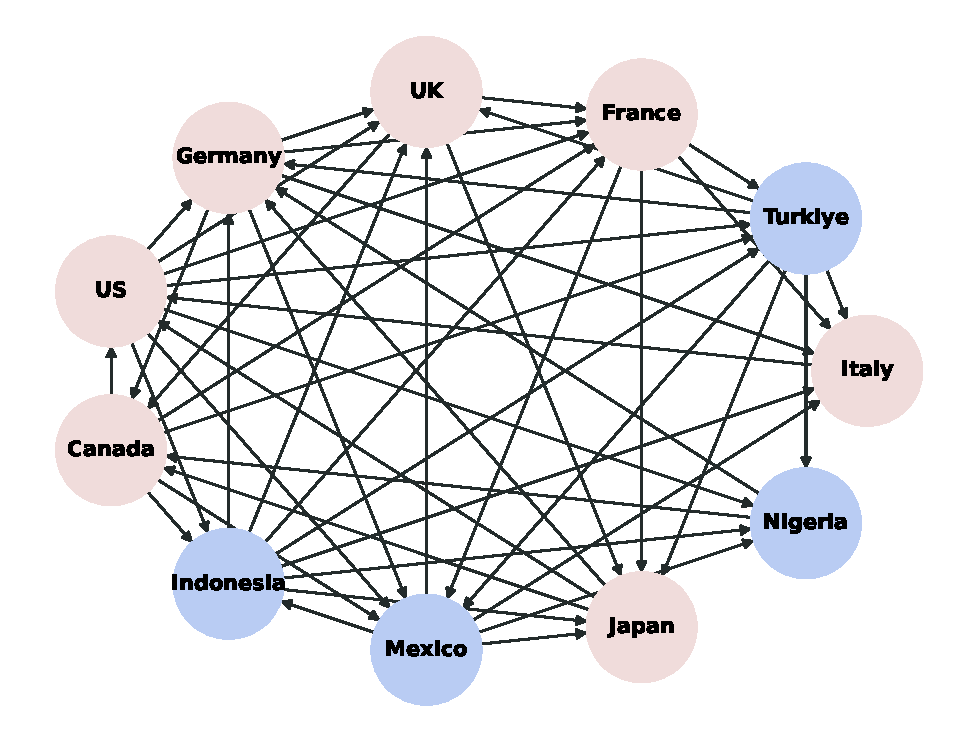
\includegraphics[width=0.48\textwidth]{./figures/graph.eps}
  \caption{The connectivity of the countries' stock indices deduced by the MTGNN.} 
  \label{fig:graph}
\end{figure}


The results in Table~\ref{tab:comparison} show that the performance of the MTGNN is excellent across 
all the stock indices of MINT and G7 countries that we considered, with RSE, RMSE, MAE, and MAPE evaluation metrics. When evaluating the second-best results in Table~\ref{tab:comparison}, it is obvious that on contrary to MTGNN, the other deep-learning methods RNN-GRU \textit{(second-best model for 2 countries' indices - Italy, Germany)} and TCN \textit{(second-best model for 3 countries' indices - T\"{u}rkiye, Japan, Nigeria)}, are not as successful as VAR-MLP \textit{(second-best model for 5 countries' indices - France, US, Canada, Indonesia, Mexico)}.

We also have provided a plot of the predictions of the MTGNN, as it is applied to the dataset we set out 
to test the trained parameters (see Figure~\ref{fig:predictions}).  The plots in Figure~\ref{fig:predictions} visually show the 
performance of the MTGNN in predicting the closing prices of each country's stock indices in this test data date range. The performance of the MTGNN is not only satisfactory in terms of its RSE, RMSE, MAE, and MAPE performances, but is also visually pleasing, as can be observed by perusing each plot in the figure. 

\begin{rem}
The MTGNN algorithm normalizes the data by subtracting from each column its individual mean and dividing by its individual standard deviation. All data transformations \textit{(natural logarithm and normalization)} are inverted for the construction of the plots in Figure~\ref{fig:predictions}.
\end{rem}

\setlength{\tabcolsep}{18pt}
\begin{table*}[bt]
    \caption{Comparison of performances of various algorithms from the literature.}
    \label{tab:comparison}
    \centering
    \scalebox{0.89}{
    \begin{tabular}{ *6l }           \toprule
    \textit{Index}& \textit{Algorithm} & \textit{RSE} & \textit{RMSE} & \textit{MAE} & \textit{MAPE} \\  
    \cmidrule(lr){1-6}
    \multirow{5}{*}{\hspace{-5mm}\minitab[l]{FTSE MIB \\ (Italy)}} & AR & $3.503$ & $0.276$ & $0.242$ & $2.4\%$  \\
    & VAR-MLP & $1.066$ & $0.152$ & $0.125$ & $1.2\%$ \\
    & RNN-GRU & $\underline{1.005}$ & $\underline{0.148}$ & $\underline{1.005}$ & $\underline{1.1}\%$\\
    & TCN & $1.545$ & $0.183$ & $0.174$ & $1.7\%$\\
    & MTGNN & $\textbf{0.026}$ & $\textbf{0.024}$ & \textbf{0.020} & $\textbf{0.2}\%$\\
    \midrule
    \multirow{5}{*}{\hspace{-5mm}\minitab[l]{BIST 100 \\ (T\"{u}rkiye)}} & AR & $10.294$ & $1.672$ & $1.600$ & $18.4\%$ \\
    & VAR-MLP & $1.487$ & $0.633$ & $0.558$ & $6.4\%$ \\
    & RNN-GRU & $0.890$ & $0.492$ & $0.428$ & $4.9\%$\\
    & TCN & $\underline{0.439}$ & $\underline{0.346}$ & $\underline{0.331}$ & $\underline{3.8}\%$ \\
    & MTGNN & $\textbf{0.081}$& $\textbf{0.042}$ & $\textbf{0.033}$ & $\textbf{0.4}\%$ \\
    \midrule
    \multirow{5}{*}{\hspace{-5mm}\minitab[l]{CAC 40 \\ (France)}} & AR & $6.939$ & $0.237$ & $0.227$ & $2.6\%$ \\
    & VAR-MLP & $\underline{0.980}$ & $\underline{0.089}$ & $\underline{0.076}$ & $\underline{0.9}\%$ \\
    & RNN-GRU & $5.589$ & $0.213$ & $0.184$ & $2.1\%$\\
    & TCN & $2.246$ & $0.135$ & $0.133$ & $1.5\%$\\
    & MTGNN & $\textbf{0.045}$ & $\textbf{0.020}$ & $\textbf{0.017}$ & $\textbf{0.2}\%$\\
    \midrule
    \multirow{5}{*}{\hspace{-5mm}\minitab[l]{FTSE 100 \\ (UK)}} & AR & $\underline{0.872}$ & $\underline{0.040}$ & $\underline{0.031}$ & $\underline{0.3}\%$\\
    & VAR-MLP & $1.562$ & $0.053$ & $0.046$ & $0.5\%$ \\
    & RNN-GRU & $6.76$ & $0.111$ & $0.093$ & $1.0\%$\\
    & TCN & $10.208$ & $0.136$ & $0.133$ & $1.5\%$\\
    & MTGNN & $\textbf{0.044}$ & $\textbf{0.018}$ & $\textbf{0.016}$ & $\textbf{0.2}\%$\\
    \midrule
    \multirow{5}{*}{\hspace{-5mm}\minitab[l]{DAX PERFORMANCE \\ (Germany)}} & AR & $2.891$ & $0.192$ & $0.175$ & $1.8\%$ \\
    & VAR-MLP & $1.017$ & $0.114$ & $0.092$ & $0.9\%$ \\
    & RNN-GRU & $\underline{0.405}$ & $\underline{0.072}$ & $\underline{0.047}$ & $\underline{0.5}\%$\\ 
    & TCN & $2.706$ & $0.169$ & $0.124$ & $1.9\%$\\
    & MTGNN & $\textbf{0.032}$ & $\textbf{0.023}$ & $\textbf{0.020}$ & $\textbf{0.2}\%$\\
    \midrule
    \multirow{5}{*}{\hspace{-5mm}\minitab[l]{S\&P 500 \\ (US)}} & AR & $10.008$ & $0.357$ & $0.346$ & $4.1\%$ \\
    & VAR-MLP & $\underline{0.965}$ & $\underline{0.111}$ & $\underline{0.092}$ & $\underline{1.1}\%$ \\
    & RNN-GRU & $2.879$ & $0.192$ & $0.157$ & $1.9\%$\\
    & TCN & $2.241$ & $0.169$ & $0.163$ & $1.9\%$ \\
    & MTGNN & $\textbf{0.031}$ & $\textbf{0.021}$ & $\textbf{0.018}$ & $\textbf{0.2}\%$\\
    \midrule
    \multirow{5}{*}{\hspace{-5mm}\minitab[l]{S\&P/TSX \\ (Canada)}}& AR & $16.568$ & $0.209$ & $0.203$ & $2.0\%$ \\
    & VAR-MLP & $\underline{1.104}$ & $\underline{0.054}$ & $\underline{0.043}$ & $\underline{0.4}\%$ \\
    & RNN-GRU & $51.66$ & $0.368$ & $0.337$ & $3.4\%$\\
    & TCN & $5.929$ & $0.125$ & $0.124$ & $1.3\%$\\
    & MTGNN & $\textbf{0.024}$ & $\textbf{0.020}$ & $\textbf{0.017}$ & $\textbf{0.2}\%$\\
    \midrule
    \multirow{5}{*}{\hspace{-5mm}\minitab[l]{IDX COMPOSITE\\ (Indonesia)}} & AR & $2.812$ & $0.050$ & $0.040$ & $0.5\%$ \\
    & VAR-MLP & $\underline{1.111}$ & $\underline{0.031}$ & $\underline{0.027}$ & $\underline{0.3}\%$ \\
    & RNN-GRU & $17.536$ & $0.124$ & $0.117$ & $1.3\%$\\
    & TCN & $66.671$ & $0.241$ & $0.231$ & $2.61\%$ \\
    & MTGNN & $\textbf{0.037}$ & $\textbf{0.016}$ & $\textbf{0.014}$ & $\textbf{0.2}\%$\\
    \midrule
    \multirow{5}{*}{\hspace{-5mm}\minitab[l]{IPC MEXICO\\ (Mexico)}} & AR & $6.134$ & $0.152$ & $0.140$ & $1.3\%$ \\
    & VAR-MLP & $\underline{0.987}$ & $\underline{0.061}$ & $\underline{0.048}$ & $\underline{0.4}\%$ \\
    & RNN-GRU & $1.526$ & $0.076$ & $0.068$ & $0.6\%$\\
    & TCN & $7.981$ & $0.173$ & $0.163$ & $1.5\%$\\
    & MTGNN & $\textbf{0.021}$ & $\textbf{0.022}$ & $\textbf{0.018}$ & $\textbf{0.2}\%$\\
    \midrule
    \multirow{5}{*}{\hspace{-5mm}\minitab[l]{NIKKEI 225 \\ (Japan)}} & AR & $5.273$ & $0.329$ & $0.315$ & $3.0\%$ \\
    & VAR-MLP & $1.597$ & $0.181$ & $0.160$ & $1.6\%$ \\
    & RNN-GRU & $1.654$ & $0.184$ & $0.148$ & $1.4\%$\\
    & TCN & $\underline{0.298}$ & $\underline{0.078}$ & $\underline{0.075}$ & $\underline{0.7}\%$\\
    & MTGNN & $\textbf{0.025}$ & $\textbf{0.025}$ & $\textbf{0.020}$ & $\textbf{0.2}\%$\\
    \midrule
    \multirow{5}{*}{\hspace{-5mm}\minitab[l]{NSE 30 \\ (Nigeria)}} & AR & $6.526$ & $0.747$ & $0.700$ & $8.9\%$ \\
    & VAR-MLP & $1.190$ & $0.319$ & $0.292$ & $3.8\%$ \\
    & RNN-GRU & $0.491$ & $0.205$ & $0.128$ & $1.6\%$\\
    & TCN & $\underline{0.045}$ & $\underline{0.062}$ & $\underline{0.057}$ & $\underline{0.7}\%$\\
    & MTGNN & $\textbf{0.013}$ & $\textbf{0.026}$ & $\textbf{0.018}$ & $\textbf{0.2}\%$ \\
    \bottomrule
    \hline
    \end{tabular}
    }
    \begin{tablenotes}
      \small
      \centering
      \item The best results are bolded, and the second best results are underlined.
    \end{tablenotes}
\end{table*}


\begin{figure*}[tbh]
  \centering
  % \includegraphics[width=0.45\textwidth]{./figures/.eps}
  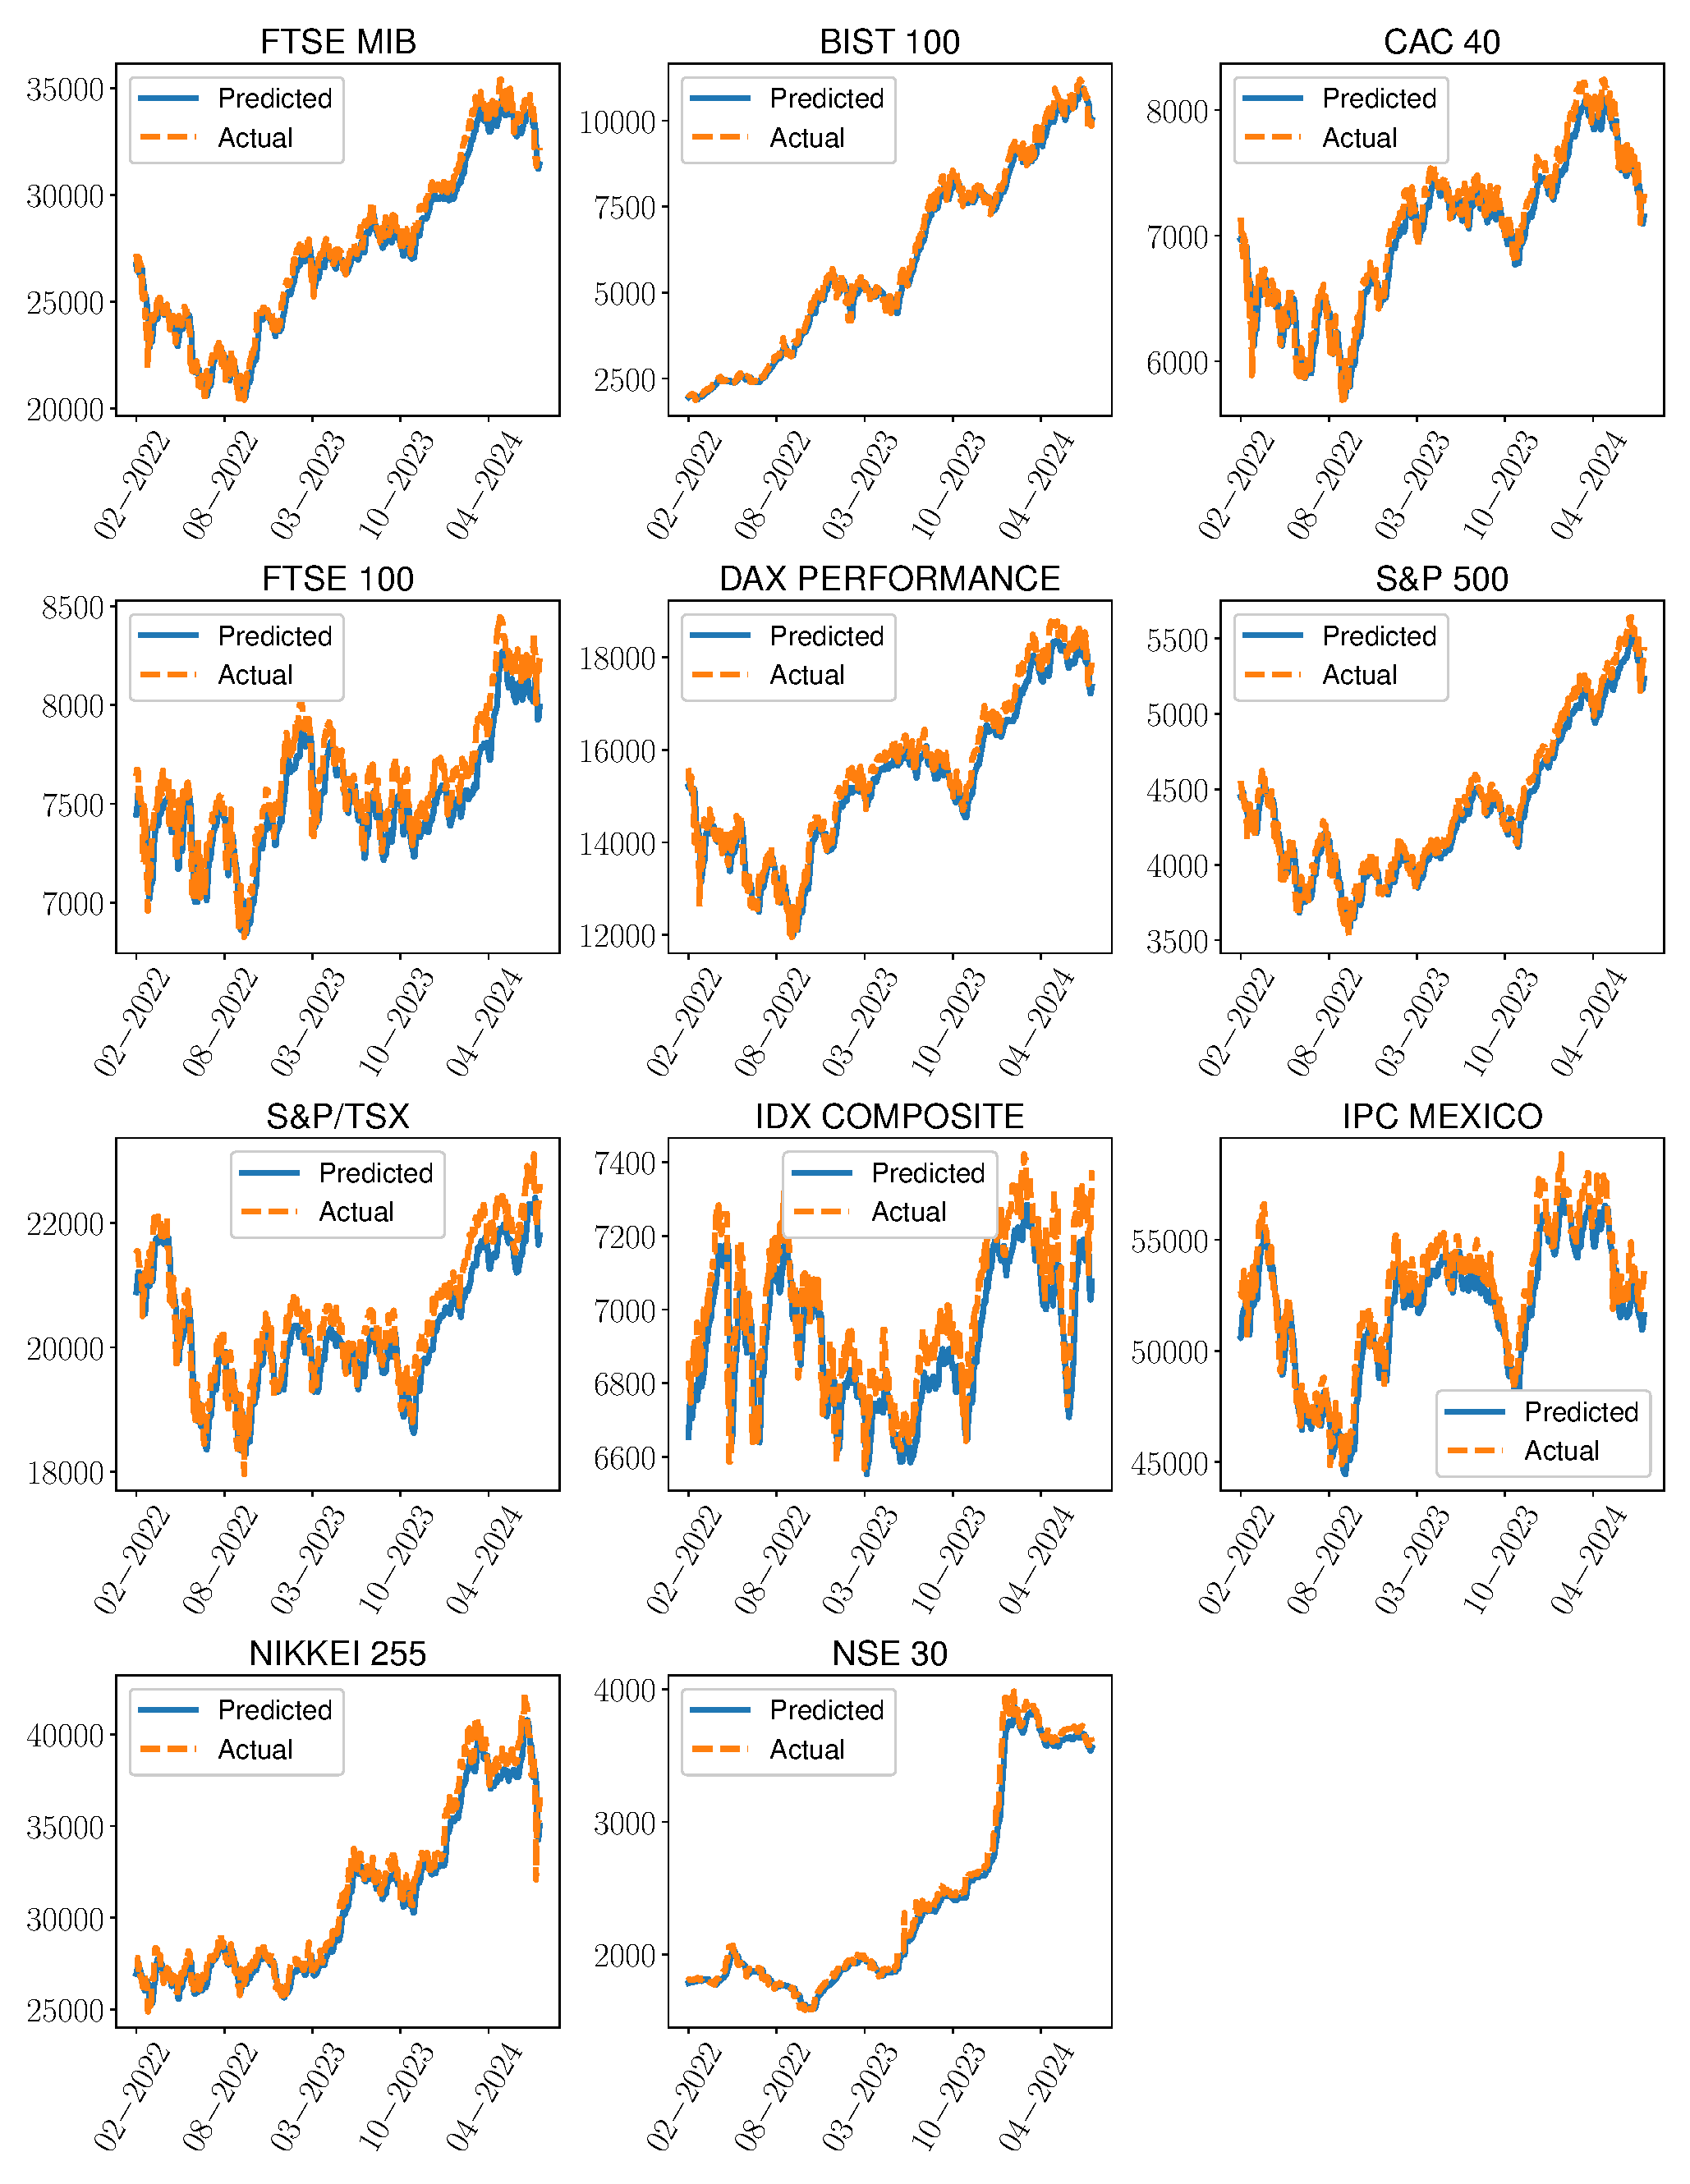
\includegraphics[width=0.97\textwidth]{./figures/predictions.eps}
  \caption{The predictions obtained MTGNN predictor.} 
  \label{fig:predictions}
\end{figure*}